\subsubsection{Catalog Page Specifications}
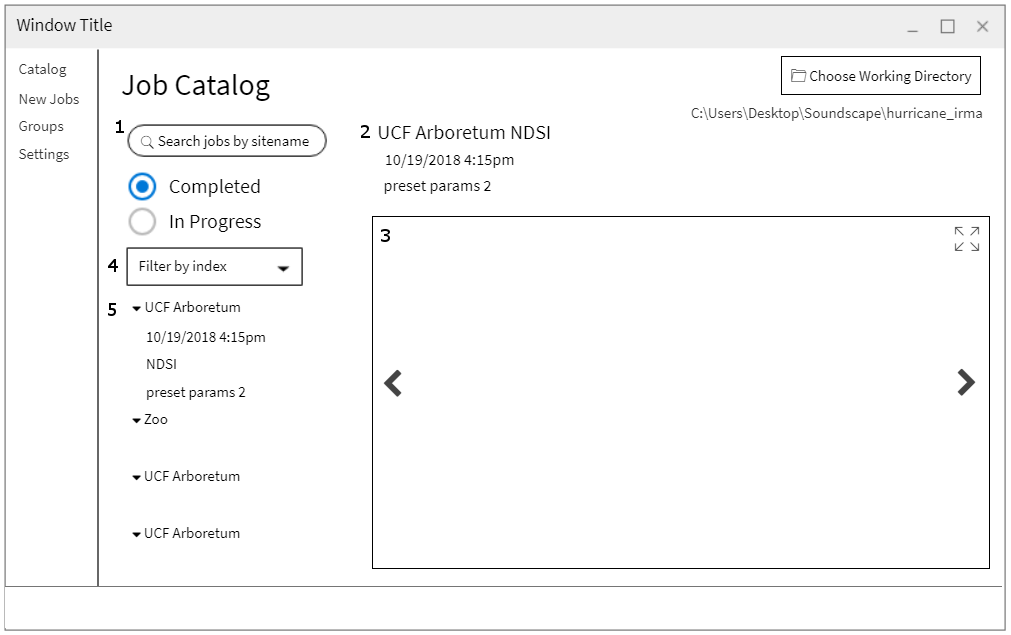
\includegraphics[width=\textwidth]{CatalogPage}
The catalog page is where the user can view their already processed data stored in the backend. If this user is using a shared server, this can potentially also show processed data from \textit{other} users in their group, should those permissions be allowed. Core functionality of the catalog page is as follows:\\
\begin{enumerate}
    \item \textbf{Job Searching}\\ The user can search for jobs by name, date, or index. Every job created by the user is given a name, the date is grabbed automatically, and the index is chosen by the user. The user can search currently processing jobs, as well as completed ones.
    \item \textbf{Selected Job Name}\\ This title is the selected job name, along with the date and time of analysis completion, and the paramters run on it.
    \item \textbf{Job Analysis}\\ This is where the analysis from the job is shown. Depending on the parameters and index that was processed, different visualizations will be available. If multiple jobs are selected, then a visualization comparing them will be shown.
    \item \textbf{Job Filtering}\\ In addition to job name searching, the user can filter jobs by their index. This will allow the user to find any job they have processed given the chosen index.
    \item \textbf{Job Search Results}\\ The jobs here are those filtered by the user either by the index filter or the search bar. These can be selected for viewing in the Job Analysis section.
\end{enumerate}